\chapter{Methods}
\label{chap:methods}


\section{Computational Methods}

\subsection{Kinetic Monte Carlo}
With each chromphore taken to be a discrete object, both in python, and with respect to its frontier
molecular orbitals, a charge hopping from an excited chromophore to a neighboring chromophore can be modeled
as a discrete event that occurs at a rate estimable by semiclassical Marcus theory. The rate that a hop will
occur from chromophore $i$ to chromophore $j$, $k_{ij}$, is given by the
following equation:

\begin{align}
    k_{ij}  =  
\end{align}

The inputs to the equation and how they are computed are in the following section. But taking k to be and
accruate rate of the electron transfer reation, we implant a charge randomely into the morhpology, calculate
the rate of all possble events(possible hops in our case)
and put them in order of quickest to slowest. The logic is, with k ranging across orders of magnitude, the
probibitly of the event happing is the inverse of k. It is assumed that hopping processes at the angtrom level
will proceed stochastically. This implementation, and other sucessful ones like it [NEED REFS?] have
implemented this via a scaling of the wait time, or inverse rate of the hop. The scaling facter is -lnx where
x is a random number between 0 and 1. This allows rare events to happen (rarely). With potentially millions of
hops this indroduces signifcant stochasticism. The waittime then looks as follows:

\begin{align}
    \tau =  -\ln{x}  \bigg( \frac{1}{k} \bigg)
\end{align}


\subsection{Quantum Chemical Methods}
At the core of Morphct is the estimation of HOMO (for donor) and LUMO (acceptor). This is because 
the inputs into the marcus hopping equation are the offsets between neighboring  chromophores energy levels
determine the driving force and the TI is estimated using a dimer method that also uses the homo level. 
With that said, quantum chemical methods give us a framework from which to estimate the homo/lumos. A litany of
methods that use approximations and parametrizations to transform cumbersome ab initio quantum mechanical 
calculations into efficient algorithms for determining the electronic structure of a given compound. Morpcht 
leverages MINDO/3, a variation of the INDO(Intermediate Neglect of Differential Overlap) method,
which is an approximation method that seeks recreate the ab initio Hartree-Fock
results, where the Hatree-Fock theory allows for an iteratively convergent numerical solution to the Shreodinger equation.\cite{Thiel2014}. Calculating electronic structure with this method has
shown good agreement with experimental data and more rigorous Quantum chemical
methods 
\cite{Bredas2002}. Furthermore, variations in TI dont effect mobilitity calcs
that much (one of evans papers said this).  Results
from the this work compare well to jones2017 which implemented ZINDO/s, another
semi-empirical method. The
previous version of MorphCT utilized ORCA to provide the quantum chemical
approximations required to implement
a hopping model of charge transport \cite{Neese2012b}. Jones2017 showed that with this you can connect MD
provided morphology to charge transport characteristics. A particular 
choice of method comes down to how well we can organize a workflow and integrate the QQC portion of the
workflow modularly. This is becuase the quantum compuational chemistry is a nascent and evolving field of its
own, with quickly increasing effeciencys and accuracies. Therefor, an important consideration is, "how can we
deintigrate and reintigrate a QCC software, tests its efficiency and accuracy, and do it in a way that lays
the groundwork to upgrade or swap it as better options emerge?". 

\indent The software chosen to implement this method is
provided by pySCF (Python-based Simulations of Chemistry Framework) \cite{Sun2018a}. This framework
was chosen in the interest of reproducability and extensibility. PySCF is implemented almost entirly in the Python 
language, which is becoming increasingly ubiquitous in the scientific computing community. Furthermore,
ORCA's proprietary licensing was prohibitive in the efforts to containerize MorphCT for use on cluster and for
creating reproducible results. 
Solving shrodingers equation across tens of thousands of 
chromophores, which will be required to model an OPV material on the order of 10 nm, is untenable. Therefore
justified but drastic simplifications are necessary. Computation of the eigenvalues of the HOMO and HOMO-1
molecular orbitals of the dimer Hamiltonian requires the computation of three integrals: 
the site energy integral, the transfer integral (electronic overlap), and the overlap integral (physical
overlap). Neglecting the latter using an implementation of an INDO method can provide an effective transfer
integral. It is this approximation that allows an estimating of the transfer integral from the calculation of
the dimer splitting energy and the site energy. A further approximation, which is more relevant for highly regular chromopheres is Koopman's
approximation, which further neglects the site energy integral, thereby assuming all chromophores have the same
energetics in isolation.  \cite{Huang2005b}. Other studies have implemented DFT at this stage of predicting
mobility from molecular arrangement to good effect \cite{Deng2004}. The P3HT morphologies discussed in the evaluation section of the results
consist of 1000 oligomers of 15 repeating molecular units. Assigning each molecular unit as a chromophore
gives 15000 indivual QQC calculations and as many as 15000 choose 2 Dimer QCC calculations. The latter is
drastically lower because not all chromophores interact. In this workflow neighbor, finding is accomplished via
voronoi analysis. Nevertheless, with the volume of calculations necasssary to simulate materials into the
nanometer range, DFT is prohibitivly slow. 

Figure blaf \ref{fig:TI} shows MorphCT calculated values the transfer integral between two thiophene
rings. Using Mbuild, a reference thiopophene is placed in the xy-plane with the y-axis running through the 
the sulfur atom and its center mass placed at the origin. A second thiophene is instantiated in the same manner but a
combination of allowable moves is created wherein the second thiophene can translate up to 5 angstroms 
and rotate up to 90 degress about its x and z axis. Center-to-center distances less than 3 angstroms are disallowed. 
This gives 4300 unique orientations show in figure \ref{ref:TI}. The figure shows that, as expected,
center-to-center distance decreasing results in more orbital overlap. Also observable in the figure is that
a rotation of 90 degrees about the x axis corresponds to the sulfer of the second thiophene being oreinted
straight towards the reference thiophene corresponds to a smaller sulfer-to-sulfler distance and a greater TI. 

It is known that the ionization potential and thus the homo-lumo gap has a near linear relationship with the
size of the chromophore. In figure \ref{fig:fused}, we can see this relationship is corroberated by our
implementation of PySCF. This phenomoena has been shown using experiment and DFT methods  \cite{Arago2010}


\begin{figure}
  \center
  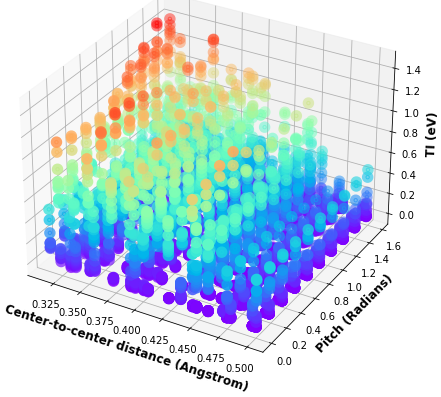
\includegraphics[width=10cm]{figures/transfer_integral_plot.png}
  \caption{Thiophene Transfer Integrals}
  \label{fig:TI}
\end{figure}
\begin{figure}
  \center
  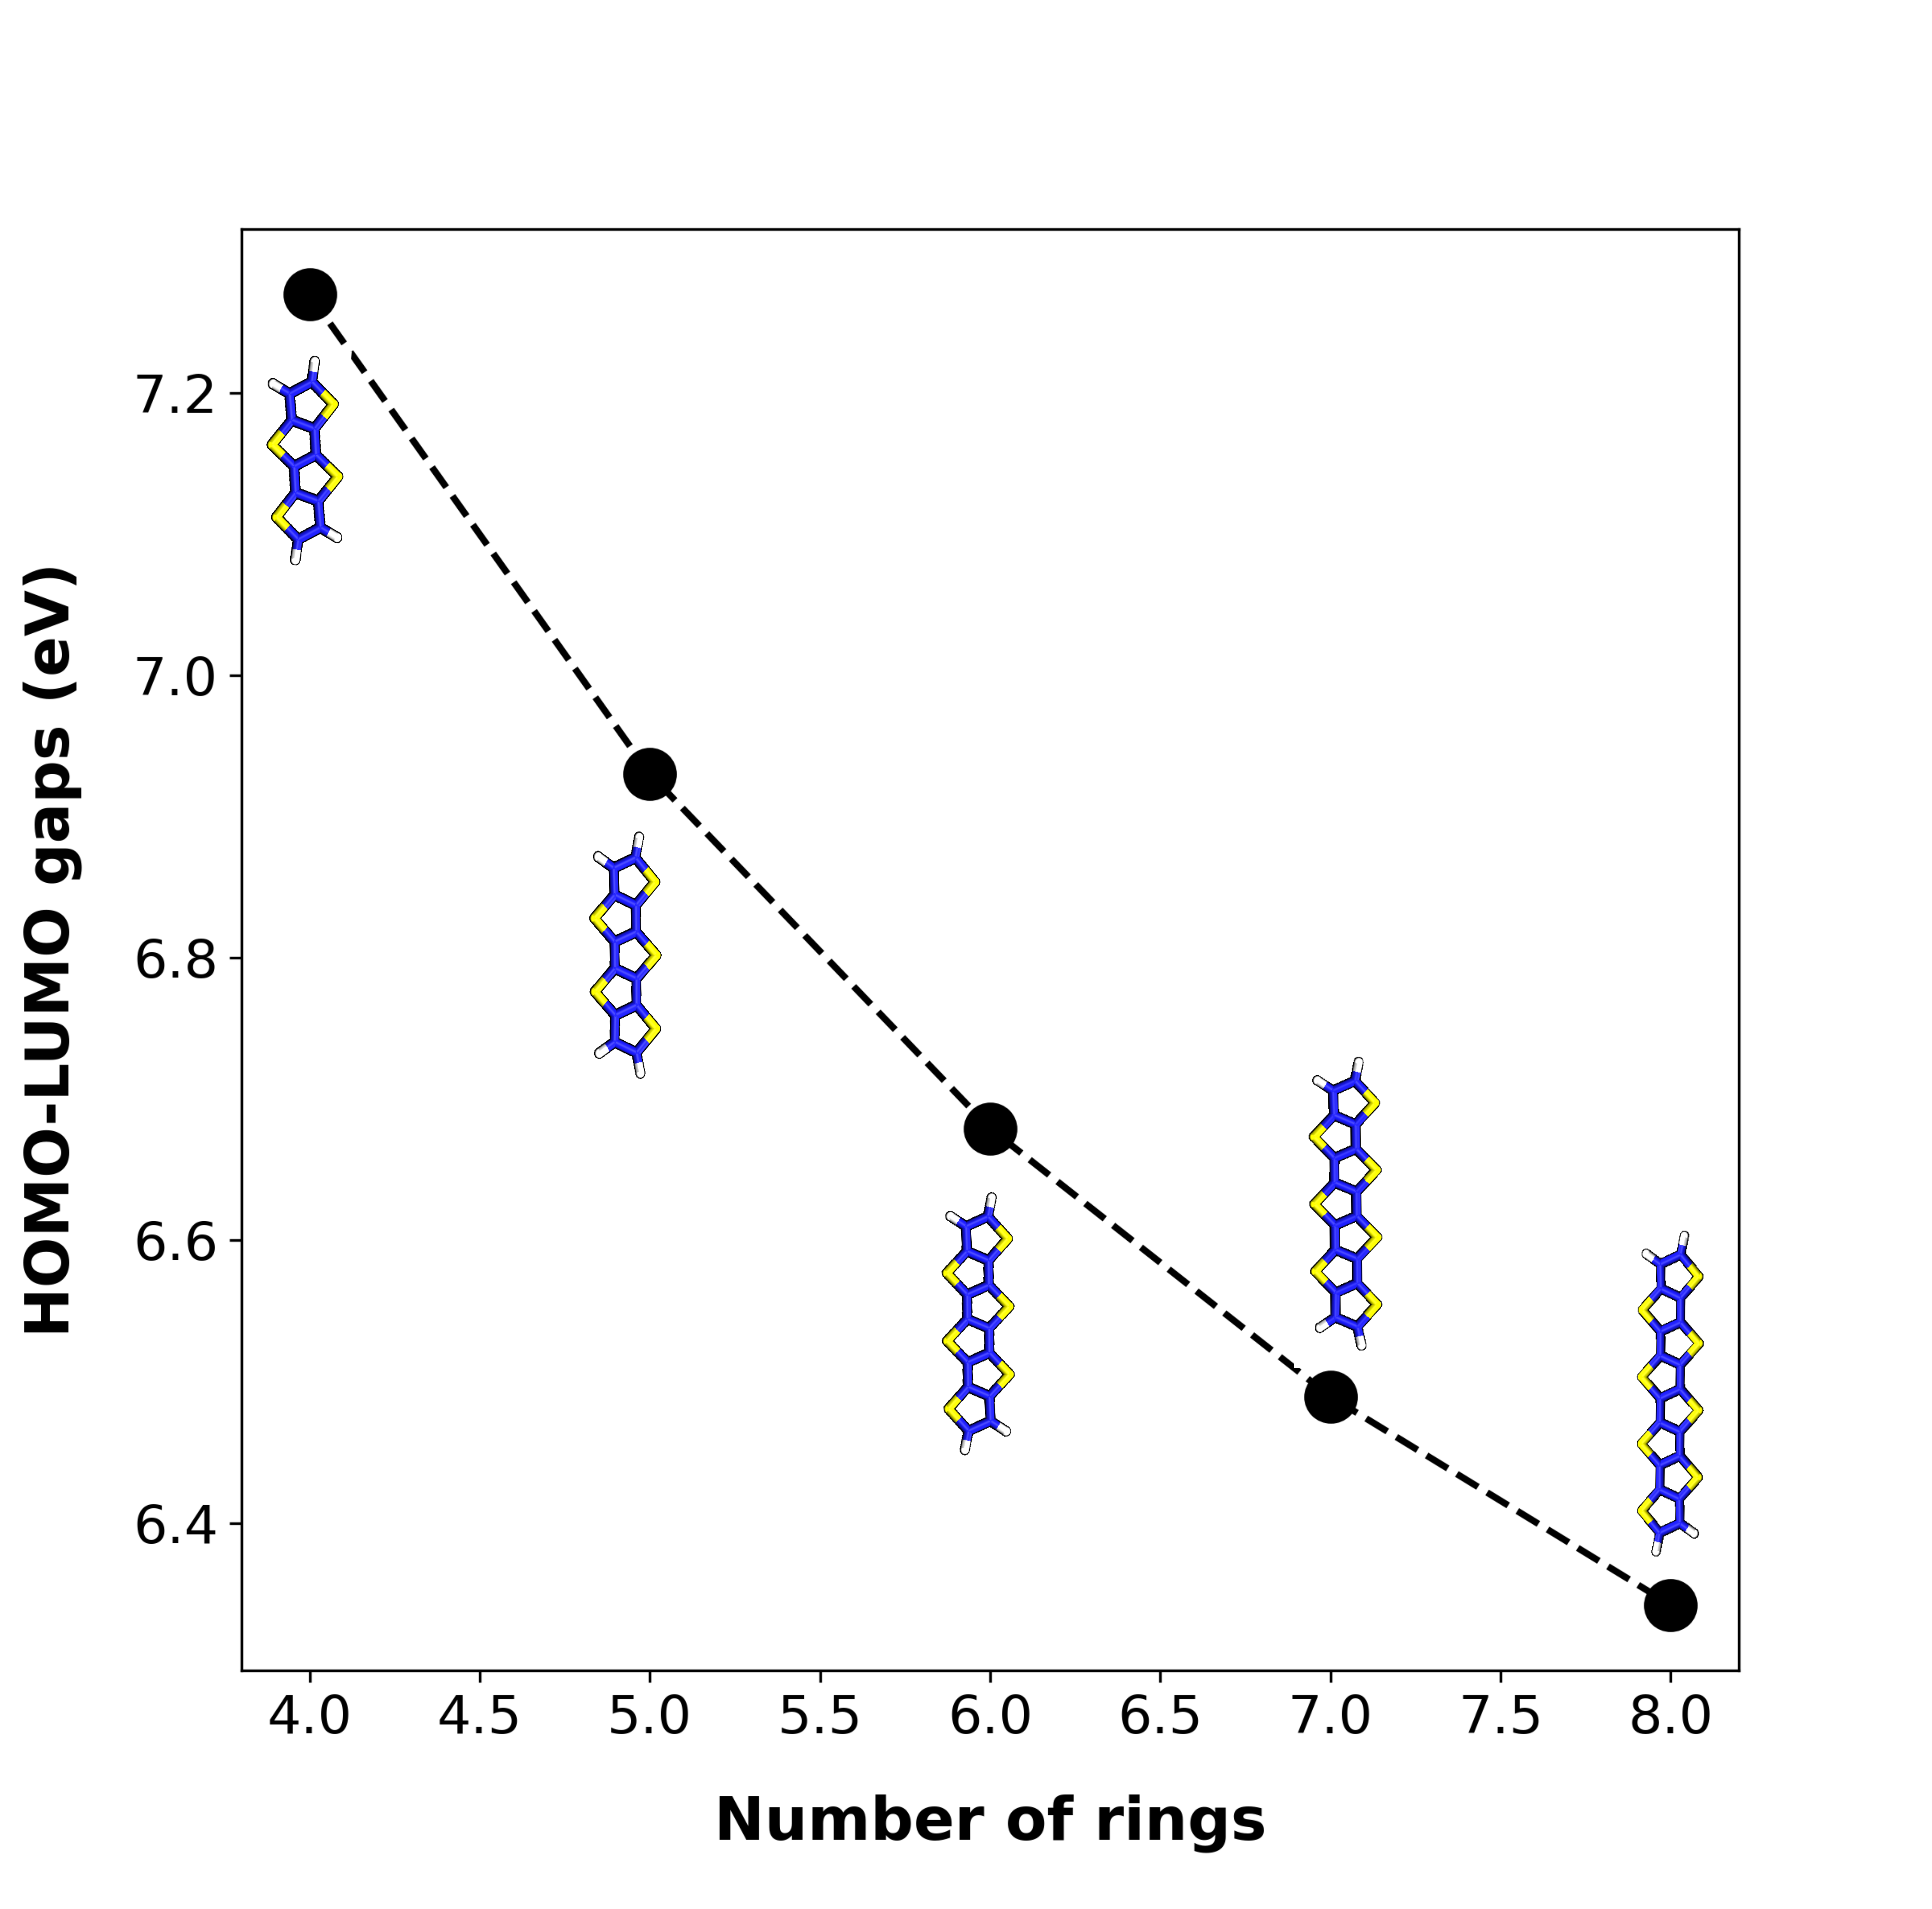
\includegraphics[width=15cm]{figures/fused-ring-figure.png}
  \caption{Thiophene Transfer Integrals}
  \label{fig:fused}
\end{figure}


\indent Graduating these pairwise energetics to charge characteristics on the scale of MD simulations
requires the use of an iterative algorithm. Implemnting a hopping simulation requires the delineation of
individual segments of delocalization or chromophores. For polymeric materials like P3HT, MorphCT
can identify chromophores with a provided SMILES string. For less regular molecules, explicitly delineating
which atoms belong to which chromophores is required. At this stage of the workflow, consideration needs to be
given to where a charge may delocalize within. With ITIC, the frontier molecular oribitals, that is, the HOMO
and LUMO have neglegible electon density along the side chains. With that, significant computational recources
can be conserved by leaving these atoms out of the of the QCC stage. To test this on ITIC we delineate the
backbone and the whole molecule and compare carrier mobility NEED THIS DATA. 

\section{\nobreak kmc analysis}
Taking a charge to be a quasi-particle inserted into a MD generated morpholgy, a KMC
simulation can be run on the bases of Marcus rates obtained from QCC.
The KMC algorithm allows an explicit calculation of the MSD accross a large number of 
particles in the system. Repeating along relevant time scales for 
charge transfer, knowing that MSD scales linearly with time, the slope of this relationship
can be estimated and related to to the 3D diffusion coeffiecient. Using the Einstien relation, 
the groundwork for which Einstein derived in his doctoral dissertaion, finally the zero-field
mobility can be obtained. 
It is critical that we not include the ballistic transport timescale in the approximation of the limit
if the slope as time goes to infinity \cite{Maginn2018} . This could be easily demonstrated by leaving $10^{-13}$ as the first
lifetime for example and show how that effects the MSD slope. Estimating an upperbound for lifetimes such that
we can estimate the slope of the MSD as time goes to infinity can be messy. In real systems, free chrage
carrier lifetime is subject to a complex interplay between geminate recombination, non-geminate recombination,
charge trapping, temperature, and charge density, whose dynamics play out accros a picosecond to microsecond
timescales and vary widly form material to material as well as from microstrtucture to microstrucute for a
given material \cite{Laquai2015} . For this work, the primary strategy was to avoid the ballistic region while exploring lifetimes
that are achievable computationally. For example, I tried to go to the physical edge of lifetimes and
calculate MSD out to a microsecond. A single hole hopped for 9 wall  time hours. It could be beneficial to do
a preanalysis in morph that estimates where a given morphology's MSD will converge so as to never simulate
past that time. To do so is superflous and expensive. 
In this work, we ignore dynamic disorder by doing calculations on snapshots from equillibrium MD simulations.
Others have had success intruducing dynamic disorder via nudging the QQC calculated TI value at every
iteration of the KMC algorithm by a number drawn randomly from a Gaussian Distribtion \cite{Gali2017}.
\subsection{Voronoi Analysis}
\begin{figure}
  \center
%\includegraphics[width=25cm]{figures/crystalline_voronoi.png}
  \includegraphics[width=\linewidth, height=\textheight,keepaspectratio]{figures/crystalline_voronoi_smaller.png} 
 % \includegraphics[width=\linewidth]{figures/crystalline_voronoi_smaller.png}
  \caption{2D Voronoi}
  \label{fig:2d}
\end{figure}


Again, with 15000 choose 2 pairs, we are required to perform some neighborlisting prior to QCC. For this we chose to
implement freud voronoi analysis. Utilizingn the freud.locality.Voronoi() so catergoriaze chromophores as
neihgbors if they share an edge in the voronoi cells around the geometric center of the chromphore. Here, the
cell edges are drawn in a Euclidean way, with lines representing the set of points equidistant from a point
and its geomerically closest neighbor across the line. This analysis takes place in three dimensions. As a
demonstration a voronoi analysis was run on a 2D analogue of the crystalline P3HT system described elsewhere.
In figure [FIGURE], 15,000 thousand dots represent the single-monomer chromophore's geometric centers projected
in the xy-plane.Here,
a voronoi cell for any given chromophore center is the set of points that are closer to that chromophore
center than any other chromopore center. We use voronoi because BLAH. Euclidean space searching algorithms of
this sort are known to scale with $O(n\log{n})$ in the worst case and as low as $O(n)$ in the average case
\cite{Bentley1980}.
However as can seen from the figure, two points can share cell edges despite being rather far apart. We
therefore, further remove pairs from the neighborlist if they are far enough apart such that it is justifyable
to assume they dont interact electronically enough to effect to charge mobility calc. This parameter will
dependend on the material under investigation as was as the size of the individual chromophores. We tested the
sensitivity of the algorithm to the value (dcut). The figure shows the effect of cutoff distance on value of
calculated mobility. there is a diminishing returns around dcut10. 
%%% Local Variables: 
%%% mode: latex
%%% TeX-master: "BSUmain"
%%% End: 
